\documentclass{article}
%%%%%%%%%%%%%%%%%%%%%%%%%%%%%%%%%%%%%%%%%
% Lachaise Assignment
% Structure Specification File
% Version 1.0 (26/6/2018)
%
% This template originates from:
% http://www.LaTeXTemplates.com
%
% Authors:
% Marion Lachaise & François Févotte
% Vel (vel@LaTeXTemplates.com)
%
% License:
% CC BY-NC-SA 3.0 (http://creativecommons.org/licenses/by-nc-sa/3.0/)
% 
%%%%%%%%%%%%%%%%%%%%%%%%%%%%%%%%%%%%%%%%%

%----------------------------------------------------------------------------------------
%	PACKAGES AND OTHER DOCUMENT CONFIGURATIONS
%----------------------------------------------------------------------------------------

\usepackage{amsmath,amsfonts,stmaryrd,amssymb,subcaption} % Math packages

\usepackage{enumerate} % Custom item numbers for enumerations

\usepackage[ruled]{algorithm2e} % Algorithms

\usepackage[framemethod=tikz]{mdframed} % Allows defining custom boxed/framed environments

\usepackage{listings} % File listings, with syntax highlighting
\lstset{
	basicstyle=\ttfamily, % Typeset listings in monospace font
}

%----------------------------------------------------------------------------------------
%	DOCUMENT MARGINS
%----------------------------------------------------------------------------------------

\usepackage{geometry} % Required for adjusting page dimensions and margins

\geometry{
	paper=a4paper, % Paper size, change to letterpaper for US letter size
	top=2cm, % Top margin
	bottom=2.5cm, % Bottom margin
	left=2cm, % Left margin
	right=2cm, % Right margin
	headheight=14pt, % Header height
	footskip=1.5cm, % Space from the bottom margin to the baseline of the footer
	headsep=1.2cm, % Space from the top margin to the baseline of the header
	%showframe, % Uncomment to show how the type block is set on the page
}

%----------------------------------------------------------------------------------------
%	FONTS
%----------------------------------------------------------------------------------------

\usepackage[utf8]{inputenc} % Required for inputting international characters
\usepackage[T1]{fontenc} % Output font encoding for international characters

\usepackage{XCharter} % Use the XCharter fonts

%----------------------------------------------------------------------------------------
%	COMMAND LINE ENVIRONMENT
%----------------------------------------------------------------------------------------

% Usage:
% \begin{commandline}
%	\begin{verbatim}
%		$ ls
%		
%		Applications	Desktop	...
%	\end{verbatim}
% \end{commandline}

\mdfdefinestyle{commandline}{
	leftmargin=10pt,
	rightmargin=10pt,
	innerleftmargin=15pt,
	middlelinecolor=black!50!white,
	middlelinewidth=2pt,
	frametitlerule=false,
	backgroundcolor=black!5!white,
	frametitle={Command Line},
	frametitlefont={\normalfont\sffamily\color{white}\hspace{-1em}},
	frametitlebackgroundcolor=black!50!white,
	nobreak,
}

% Define a custom environment for command-line snapshots
\newenvironment{commandline}{
	\medskip
	\begin{mdframed}[style=commandline]
}{
	\end{mdframed}
	\medskip
}

%----------------------------------------------------------------------------------------
%	FILE CONTENTS ENVIRONMENT
%----------------------------------------------------------------------------------------

% Usage:
% \begin{file}[optional filename, defaults to "File"]
%	File contents, for example, with a listings environment
% \end{file}

\mdfdefinestyle{file}{
	innertopmargin=1.6\baselineskip,
	innerbottommargin=0.8\baselineskip,
	topline=false, bottomline=false,
	leftline=false, rightline=false,
	leftmargin=2cm,
	rightmargin=2cm,
	singleextra={%
		\draw[fill=black!10!white](P)++(0,-1.2em)rectangle(P-|O);
		\node[anchor=north west]
		at(P-|O){\ttfamily\mdfilename};
		%
		\def\l{3em}
		\draw(O-|P)++(-\l,0)--++(\l,\l)--(P)--(P-|O)--(O)--cycle;
		\draw(O-|P)++(-\l,0)--++(0,\l)--++(\l,0);
	},
	nobreak,
}

% Define a custom environment for file contents
\newenvironment{file}[1][File]{ % Set the default filename to "File"
	\medskip
	\newcommand{\mdfilename}{#1}
	\begin{mdframed}[style=file]
}{
	\end{mdframed}
	\medskip
}

%----------------------------------------------------------------------------------------
%	NUMBERED QUESTIONS ENVIRONMENT
%----------------------------------------------------------------------------------------

% Usage:
% \begin{question}[optional title]
%	Question contents
% \end{question}

\mdfdefinestyle{question}{
	innertopmargin=1.2\baselineskip,
	innerbottommargin=0.8\baselineskip,
	roundcorner=5pt,
	nobreak,
	singleextra={%
		\draw(P-|O)node[xshift=1em,anchor=west,fill=white,draw,rounded corners=5pt]{%
		Question \theQuestion\questionTitle};
	},
}

\newcounter{Question} % Stores the current question number that gets iterated with each new question

% Define a custom environment for numbered questions
\newenvironment{question}[1][\unskip]{
	\bigskip
	\stepcounter{Question}
	\newcommand{\questionTitle}{~#1}
	\begin{mdframed}[style=question]
}{
	\end{mdframed}
	\medskip
}

%----------------------------------------------------------------------------------------
%	WARNING TEXT ENVIRONMENT
%----------------------------------------------------------------------------------------

% Usage:
% \begin{warn}[optional title, defaults to "Warning:"]
%	Contents
% \end{warn}

\mdfdefinestyle{warning}{
	topline=false, bottomline=false,
	leftline=false, rightline=false,
	nobreak,
	singleextra={%
		\draw(P-|O)++(-0.5em,0)node(tmp1){};
		\draw(P-|O)++(0.5em,0)node(tmp2){};
		\fill[black,rotate around={45:(P-|O)}](tmp1)rectangle(tmp2);
		\node at(P-|O){\color{white}\scriptsize\bf !};
		\draw[very thick](P-|O)++(0,-1em)--(O);%--(O-|P);
	}
}

% Define a custom environment for warning text
\newenvironment{warn}[1][Warning:]{ % Set the default warning to "Warning:"
	\medskip
	\begin{mdframed}[style=warning]
		\noindent{\textbf{#1}}
}{
	\end{mdframed}
}

%----------------------------------------------------------------------------------------
%	INFORMATION ENVIRONMENT
%----------------------------------------------------------------------------------------

% Usage:
% \begin{info}[optional title, defaults to "Info:"]
% 	contents
% 	\end{info}

\mdfdefinestyle{info}{%
	topline=false, bottomline=false,
	leftline=false, rightline=false,
	nobreak,
	singleextra={%
		\fill[black](P-|O)circle[radius=0.4em];
		\node at(P-|O){\color{white}\scriptsize\bf i};
		\draw[very thick](P-|O)++(0,-0.8em)--(O);%--(O-|P);
	}
}

% Define a custom environment for information
\newenvironment{info}[1][Info:]{ % Set the default title to "Info:"
	\medskip
	\begin{mdframed}[style=info]
		\noindent{\textbf{#1}}
}{
	\end{mdframed}
}
 % Include the file specifying the document structure and custom commands
\setlength\parindent{0pt}
\usepackage[]{algorithm2e}
\usepackage{algpseudocode}

\title{EECS 545: Homework \#3} % Title of the assignment

\author{Mingliang Duanmu\\ \texttt{duanmuml@umich.edu}} % Author name and email address

\date{\today} % University, school and/or department name(s) and a date

\begin{document}

\maketitle % Print the title

\section{MAP estimates and weight decay}

Take the log of both weights, we have
$$\mathbf{w}_{ML} = \underset{\mathbf{w}}{\operatorname{argmax}} \sum_{i=1}^{N} \log (p(y^{(i)} \mid \mathbf{x}^{(i)} ; \mathbf{w}))$$
$$\mathbf{w}_{MAP} = \underset{\mathbf{w}}{\operatorname{argmax}} \sum_{i=1}^{N} \log (p(y^{(i)} \mid \mathbf{x}^{(i)} ; \mathbf{w})) + \log(p(\mathbf{w}))$$
Since $\mathbf{w} \sim \mathcal{N}(0, \tau^{2} I)$,
$$
\begin{aligned}
\log(p(\mathbf{w})) = & \log(\mathcal{N}(0, \tau^2 I)) \\
= & \log(\frac{1}{\sqrt{2\pi} \tau}) + \log(\exp(-\frac{1}{2}(\mathbf{w}^T (\tau^{-1} I)^{-1} \mathbf{w})^2)) \\ 
= & \log(\frac{1}{\sqrt{2\pi} \tau}) + \log(\exp(-\frac{\tau}{2}\mathbf{w}^T \mathbf{w})) \\
= & \log(\frac{1}{\sqrt{2\pi} \tau}) - \frac{\tau}{2}||\mathbf{w}||^2
\end{aligned}
$$
So we can rewrite $\mathbf{w}_{MAP}$ as
$$\mathbf{w}_{MAP} = \underset{\mathbf{w}}{\operatorname{argmax}} \sum_{i=1}^{N} \log (p(y^{(i)} \mid \mathbf{x}^{(i)} ; \mathbf{w})) - \frac{\tau}{2}||\mathbf{w}||^2$$
Due to the regularized term, the distance of $\mathbf{w}_{MAP}$ to zero need to be closer than $\mathbf{w}_{ML}$ to maximize the formula. Therefore, we conclude
$$||\mathbf{w}_{MAP}||_2 \leq ||\mathbf{w}_{ML}||_2$$

\section{Direct construction of valid kernels}

We assume
$$K^{(n)}_{ij} = k_n(x_i, z_j) \text{ and } K_{ij} = k(x_i, z_j)$$
where $k_n$ is a kernel so $\mathbf{K}^{(n)}$ is symmetric and positive semi-definite, in this case we judge if $k$ is a kernel.

\subsection*{a}

$$z^T \mathbf{K} z = z^T (\mathbf{K}^{(1)} + \mathbf{K}^{(2)}) z = z^T (\mathbf{K}^{(1)} + \mathbf{K}^{(2)}) z = z^T \mathbf{K}^{(1)}z + z^T \mathbf{K}^{(2)} z \geq 0$$
Therefore, $k(\mathbf{x}, \mathbf{z})$ is a kernel.

\subsection*{b}

$k(\mathbf{x}, \mathbf{z})$ is not a kernel. Suppose $\mathbf{K}^{(1)} = 0$ and $\mathbf{K}^{(2)} = 1$,
$$z^T \mathbf{K} z = z^T (\mathbf{K}^{(1)} - \mathbf{K}^{(2)}) z = - z^T z \leq 0$$

\subsection*{c}

$$z^T \mathbf{K} z = z^T (a \mathbf{K}^{(1)}) z = a z^T \mathbf{K}^{(1)} z \geq 0$$
Therefore, $k(\mathbf{x}, \mathbf{z})$ is a kernel.

\subsection*{d}

$k(\mathbf{x}, \mathbf{z})$ is not a kernel. Suppose $\mathbf{K}^{(1)} = 1$,
$$z^T \mathbf{K} z = z^T (-a \mathbf{K}^{(1)}) z =  - a z^T z \leq 0$$

\subsection*{e}

$$z^T \mathbf{K} z = \sum_{i, j} z_i K^{(1)}_{ij} K^{(2)}_{ij} z_j$$
Since $\mathbf{K}^{(1)}$ is positive semi-definite, we have
$$\mathbf{K}^{(1)} = X \varLambda X^T =\sum_{k=1}^{n} (\lambda_k X_k X_k^T)$$
where $\lambda_i \geq 0$. So
$$K^{(1)}_{i,j} = \sum_{k=1}^{n} \lambda X_{k,i} X_{k, j}$$
We have
$$
\begin{aligned}
z^T \mathbf{K} z = & \sum_{i, j} z_i K^{(1)}_{ij} K^{(2)}_{ij} z_j \\
= & \sum_{i, j} z_i \sum_{k=1}^{n} \lambda X_{k,i} X_{k, j} K^{(2)}_{ij} z_j \\
= & \sum_{k=1}^{n} (\lambda_k \sum_{i,j} z_i X_{k,i} K^{(2)}_{ij} X_{k,j} z_j)
\end{aligned}
$$
Since $\mathbf{K}^{(2)}$ is also positive semi-definite,
$$z^T \mathbf{K} z = \sum_{k=1}^{n} (\lambda_k \sum_{i,j} z_i X_{k,i} K^{(2)}_{ij} X_{k,j} z_j) \geq 0$$
Therefore, $k(\mathbf{x}, \mathbf{z})$ is a kernel.

\subsection*{f}

$$
\begin{aligned}
z^T \mathbf{K} z = & \sum_{i} \sum_{j} z_i k(x_i, x_j) z_j \\
= & \sum_{i} \sum_{j} z_i f(x_i) f(x_j) z_j \\
= & \sum_{i} (f(x_i)z_i)^2 \geq 0
\end{aligned}
$$
Therefore, $k(\mathbf{x}, \mathbf{z})$ is a kernel.

\subsection*{g}

Since $k_{3}$  is a kernel over $\mathbb{R}^{M} \times \mathbb{R}^{M}$ and $\phi: \mathbb{R}^{D} \rightarrow \mathbb{R}^{M}$, we have
$$\mathbf{K}^{(3)}_{ij} = k_3(x_i, z_j)$$
Therefore, $k(\mathbf{x}, \mathbf{z})$ is a kernel.

\subsection*{h}

$$z^T \mathbf{K} z = \sum_{i} \sum_{j} z_i p(K^{(1)}_{ij}) z_j$$
Since $p(K^{(1)}_{ij})$ is a polynomial with positive coefficients, according to the conclusions in \textbf{a}, \textbf{c}, \textbf{e}, $k(\mathbf{x}, \mathbf{z})$ is a kernel.

\subsection*{i}

Since $D = 2$, we have
$$(\mathbf{x}^T z + 1)^2 = (x_1z_1 + x_2z_2 + 1)^2 = x_1^2z_1^2 + x_2^2z_2^2 + 1 + 2x_1z_1x_1z_1 + 2x_1z_1 + 2x_2z_2$$
So we can construct a map of
$$\phi(x) = (x_1^2, x_2^2, \sqrt{2}x_1x_2, \sqrt{2}x_1, \sqrt{2}x_2 ,1)^T$$

\section{Kernelizing the Perceptron}

\subsection*{a}

\subsubsection*{i}

If $y^{(n)}h \geq 0$, $\mathbf{w}_{t+1} = \mathbf{w}_{t}$, which is in the form of $\Phi^T\mathbf{\alpha}_{t+1}$. \\
If $y^{(n)}h < 0$, $\mathbf{w}_{t+1} = \mathbf{w} + y^{(n)}\Phi(x^{(n)}) = \Phi^T\mathbf{\alpha}_{t} + y^{(n)}\Phi^Te_n$ where $e_n=(0,0,\cdots,1,0,0,\cdots)$. Therefore we have $\mathbf{w}_{t+1} = \Phi^T(\mathbf{\alpha}_t + y^{(n)}e_n)$

\subsubsection*{ii}

We initialize $\mathbf{w}_0 = \Phi^T \mathbf{\alpha}_t = 0$ where $\mathbf{\alpha}_t = 0$. \\
When $t = 0$, if $y^{(n)}h \geq 0$, then $\mathbf{w}_1 = 0$; if $y^{(n)}h < 0$, $\mathbf{w}_1 = y^{(i)} \Phi^T e_1$, which is the in the form of $\Phi^T \mathbf{\alpha}_t$. \\
We assume $\mathbf{w}_t$ is in the form of $\Phi^T \mathbf{\alpha}_t$, from the conclusion of \textbf{i} we know that $\mathbf{w}_{t+1}$ is also of the form $\Phi^T \mathbf{\alpha}_{t+1}$. \\
Therefore, we prove the conclusion by induction.

\subsection*{b}

\subsubsection*{i}

From the solution of \textbf{a}, we find: \\
For $y^{(n)}h \geq 0$, $\mathbf{\alpha}_{t+1} = \mathbf{\alpha}_t, \mathbf{w}_{t+1} = \mathbf{w}_t$. \\
For $y^{(n)}h < 0$,  $\mathbf{\alpha}_{t+1} = \mathbf{\alpha}_t + y^{(n)}e_n, \mathbf{w}_{t+1} = \mathbf{w}_t + \Phi^T y^{(n)}e_n$. \\
The maximum number of elements that differ between $\mathbf{\alpha}_t$ and $\mathbf{\alpha}_{t+1}$ is 1.

\subsubsection*{ii}

$$
\begin{aligned}
h(\phi(\boldsymbol{x}^{(n)}), \boldsymbol{w}_{t}) &=\boldsymbol{w}_{t}^{T} \phi(\boldsymbol{x}^{(n)}) = \mathbf{\alpha}_{t}^{T} \Phi \phi(\boldsymbol{x}^{(n)}) \\
&=\sum_{i=1}^{N} \mathbf{\alpha}_{t, i} \phi(\boldsymbol{x}^{(i)}) \phi(\boldsymbol{x}^{(n)}) \\
&=\sum_{i=1}^{N} \mathbf{\alpha}_{t, i} k(\boldsymbol{x}^{(i)}, \boldsymbol{x}^{(n)})
\end{aligned}
$$

\subsection*{c}

\begin{algorithm}[H]
    \caption{PERCEPTRON TRAINING ALGORITHM}
    $\alpha_0 \gets 0$; \\
    for t = 0 to T - 1 do \\
    \quad Pick a random training example $(x^{(n)}, y^{(n)})$ from D (with replacement) \\
    \quad $h \gets \sum_{i=1}^{N} \alpha_{t,i}k(x^{(i)}, x^{(n)})$ \\
    \quad if $y^{(n)}h < 0$ then \\
    \quad \quad $\alpha_{t+1} \gets \alpha_t + y^{(n)}e_n$ \\
    \quad End \\
    End \\
return $\alpha_t$
\end{algorithm}
To classify the data, we need to calculate $sign(\sum_{i=1}^{N} \alpha_{t,i}k(x^{(i)}, x^{(n)}))$ for the test data.

\section{Implementing Soft Margin SVM by Optimizing Primal Objective}

\subsection*{a}

Since
$$t^{(i)}(\boldsymbol{w}^{T} \boldsymbol{x}^{(i)}+b) \geq 1-\xi_{i}$$
where $\xi_{i} \geq 0, \forall i=1, \ldots, N$, we have
$$\xi_i \geq 1- t^{(i)}(\boldsymbol{w}^{T} \boldsymbol{x}^{(i)}+b)$$
Rewrite the expression, we set the minimum of $\xi_i$ as
$$\xi_i = \max(0, 1-t^{(i)}(\boldsymbol{w}^{T} \boldsymbol{x}^{(i)}+b))$$
Now we get the latter equation from the former one. \\
For the reverse case, the process is the same, so we prove that both equations are indeed equivalent optimization problems.

\subsection*{b}

Since 
$$\frac{\partial}{\partial x} \max(0, f(x))= \mathbf{I} \frac{\partial f(x)}{\partial x}$$
We have
$$
\begin{aligned}
\nabla_{\mathbf{w}} E(\mathbf{w}, b) = & \frac{\partial}{\partial \mathbf{w}} (\frac{1}{2}\|\mathbf{w}\|^{2}+C \sum_{i=1}^{N} \max (0,1-y^{(i)}(\mathbf{w}^{T} \mathbf{x}^{(i)}+b))) \\
= & \mathbf{w}-C \sum_{i=1}^{N} \mathbf{I}[y^{(i)}(\mathbf{w}^{T} \mathbf{x}^{(i)}+b)<1] y^{(i)} \mathbf{x}^{(i)}
\end{aligned}
$$
Similarly we have
$$
\begin{aligned}
\frac{\partial}{\partial b} E(\mathbf{w}, b) = & \frac{\partial}{\partial b} (\frac{1}{2}\|\mathbf{w}\|^{2}+C \sum_{i=1}^{N} \max (0,1-y^{(i)}(\mathbf{w}^{T} \mathbf{x}^{(i)}+b))) \\
= & -C \sum_{i=1}^{N} \mathbf{I}[y^{(i)}(\mathbf{w}^{T} \mathbf{x}^{(i)}+b)<1] y^{(i)}
\end{aligned}
$$

\newpage

\subsection*{c}

\begin{figure}[htbp]
    \centering
    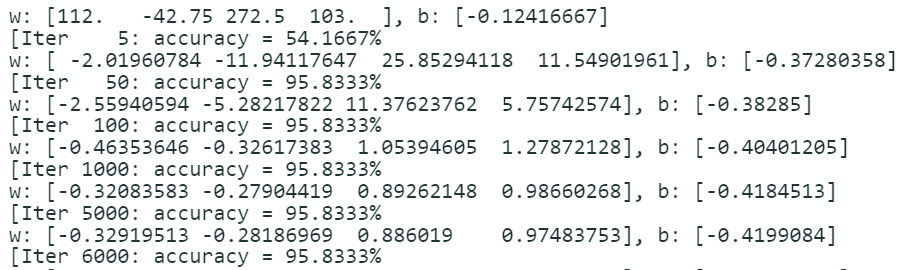
\includegraphics[width=.75\textwidth]{q4c.png}
\end{figure}

\subsection*{d}

Similarly, we have
$$\nabla_{\mathbf{w}} E^{(i)}(\mathbf{w}, b) = \frac{\mathbf{w}}{N} - C \mathbf{I}[y^{(i)}(\mathbf{w}^{T} \mathbf{x}^{(i)}+b)<1] y^{(i)} \mathbf{x}^{(i)}$$
$$\frac{\partial}{\partial b} E^{(i)}(\mathbf{w}, b) = - C \mathbf{I}[y^{(i)}(\mathbf{w}^{T} \mathbf{x}^{(i)}+b)<1] y^{(i)}$$

\subsection*{e}

\begin{figure}[htbp]
    \centering
    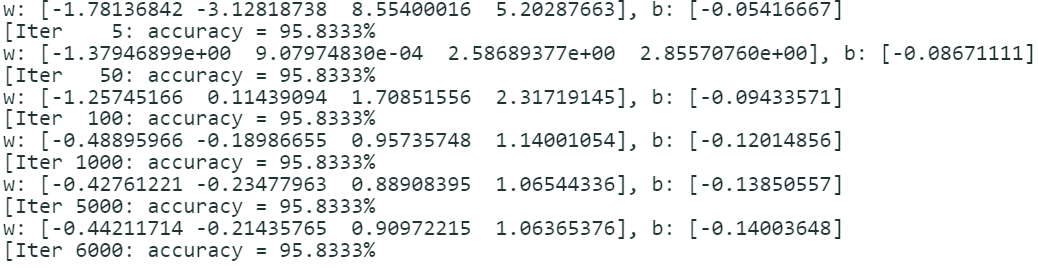
\includegraphics[width=.8\textwidth]{q4e.png}
\end{figure}

\newpage

\section{SciKit-Learn SVM for classifying SPAM}

\subsection*{a}

\begin{figure}[htbp]
    \centering
    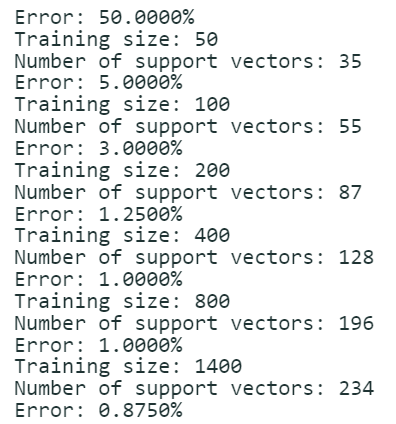
\includegraphics[width=.3\textwidth]{q5a.png}
\end{figure}

\subsection*{b}

Please check the code output of \textbf{\texttt{q5.py}} for error and number of support vectors.

\begin{figure}[htbp]
    \centering
    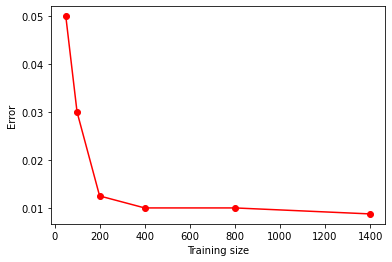
\includegraphics[width=.6\textwidth]{q5.png}
\end{figure}
The training set size of 1400 gives the best test set error.

\subsection*{c}

Compared to naive Bayes, the error of SVM is a bit higher at first when training size is small. However, with the training size increasing, SVM converges faster than naive Bayes, and the final error is smaller for large training size.
 
\end{document}